\subsection{Ejercicio 2}

Para representar el uso de 100 ciclos de CPU y dos tareas bloqueantes definimos el siguiente lote de tareas:\\

\begin{itemize}
\item TaskCPU 100 
\item TaskConsola 20 2 4
\item TaskConsola 25 2 4
\end{itemize}
TaskConsola realizará 20 y 25 llamadas bloqueantes respectivamente, con cada bloqueo de duración variable entre 2 y 4 ciclos. El cambio de contexto se fijo a 4 ciclos. En este ejercicio, el enunciado no aclaraba nada de costos de migración, con lo cual lo mantuvimos en cero. Estos fueron los gráficos obtenidos :



\begin{figure}[h]
  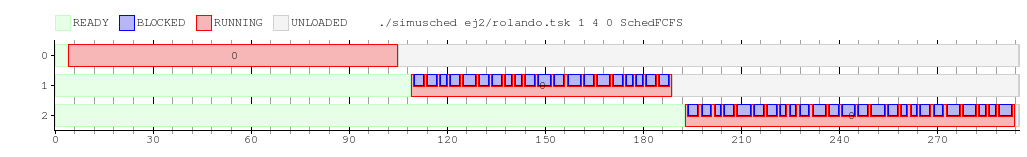
\includegraphics[width=\textwidth]{../ej2/uncore.png}
  \caption{Un núcleo.}
  \label{fig:unnucleo}
\end{figure}

La latencia es el tiempo que un proceso tarda en empezar a ejecutarse. En la figura ~\ref{fig:unnucleo}, con un núcleo, la latencia para las tareas será la suma entre el costo de cambio de contexto, la duración de la tarea anterior y la latencia de la tarea anterior. En el caso de la primer tarea (la cero) su latencia es 4, ya que no tiene tareas anteriores. La segunda tarea (la uno) tendrá latencia $ 4 + 100 + 4 = 108$. Por último, la tarea 2 tendra latencia $ 108 + duracion\_tarea_{1} + 4$. La duración de la $tarea_{1}$ viendo el gráfico es aproximadamente de 78 ciclos, con lo que su latencia es 190 ciclos.




\begin{figure}[h]
  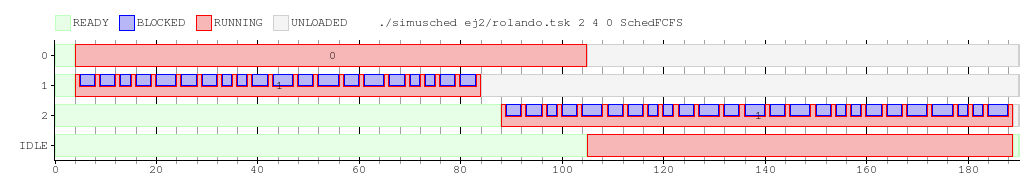
\includegraphics[width=\textwidth]{../ej2/doscores.png}
  \caption{}
  \label{fig:dosnucleos}
\end{figure}

En cambio, en la figura ~\ref{fig:dosnucleos} con dos núcleos, las tareas cero y uno tiene latencia 4, ya que ambas corren en núcleos distintos. Luego, la tarea  dos tienen latencia $4 + duracion\_tarea_{1} + 4$. La duración de la $tarea_{1}$ es de 80 ciclos, con lo que la latencia de la tarea dos es 88.\\

Dados los valores de latencia de cada tarea en ambos gráficos, concluimos que la desventaja de tener un solo núcleo es el aumento de la latencia. Todas las tareas deben esperar a que el CPU esté libre para correr, con lo cual el valor de latencia de una tarea refleja no solo su context switch, sino el tiempo de corrida y la latencia de las tareas anteriores. 

